% Pablo Baeyens (@pbaeyens)
% Email: pbaeyens31+github@gmail.com
% Licencia: CC BY-SA 3.0

%% Paquetes y configuración %

% Beamer
\PassOptionsToPackage{unicode}{hyperref}  % Evita errores con caracteres no ASCII
\PassOptionsToPackage{naturalnames}{hyperref} % tex.stackexchange.com/questions/10555
\documentclass[compress]{beamer}

% Idioma
\usepackage[spanish]{babel} % Traducciones
\usepackage[utf8]{inputenc} % Uso de caracteres UTF-8
\usepackage{lmodern}        % Fuentes de tamaño arbitrario
\usepackage[T1]{fontenc}    % Permite copiar y evita errores
\uselanguage{Spanish}       % Traducciones beamer
\languagepath{Spanish}      % (tex.stackexchange.com/questions/168208)

% Matemáticas
\usepackage{amsfonts}
\usepackage{amsmath}
\usepackage{amssymb}

% Colores
\definecolor{backg}{HTML}{F2F2F2}    % Fondo
\definecolor{title}{HTML}{bdc3d1}    % Títulos
\definecolor{comments}{HTML}{BDBDBD} % Comentarios
\definecolor{keywords}{HTML}{08388c} % Palabras clave
\definecolor{strings}{HTML}{FA5858}  % Strings
\definecolor{links}{HTML}{2C2C95}    % Enlaces
\definecolor{bars}{HTML}{045FB4}     % Barras (gráfico)

% Código
\usepackage{listings}
\lstset{
language=[LaTeX]TeX,
basicstyle=\footnotesize,
morekeywords={href,uselanguage,languagepath,column},
otherkeywords={pause,usetheme,usecolortheme,useinnertheme,titlepage,tableofcontents,subtitle},
breaklines=true,
backgroundcolor=\color{backg},
keywordstyle=\color{keywords},
commentstyle=\color{comments},
stringstyle=\color{strings},
tabsize=2,
% Acentos, ñ, ¿, ¡ (tex.stackexchange.com/questions/24528)
extendedchars=true,
literate={á}{{\'a}}1 {é}{{\'e}}1 {í}{{\'i}}1 {ó}{{\'o}}1
         {ú}{{\'u}}1 {ñ}{{\~n}}1 {¡}{{\textexclamdown}}1
         {¿}{{?`}}1
}

% Gráficos
\usepackage{pgfplots}
\pgfplotsset{width=7cm,compat=1.8} % Opciones para gráficos

% Columnas
\usepackage{multicol}

% Emoticonos
\usepackage{wasysym}

% tikz
\usepackage{tikz}
\usetikzlibrary{mindmap,trees,shadows}
\tikzset{ % Genera overlays
    invisible/.style={opacity=0},
    visible on/.style={alt={#1{}{invisible}}},
    alt/.code args={<#1>#2#3}{\alt<#1>{\pgfkeysalso{#2}}{\pgfkeysalso{#3}}},
}

%% Comandos %%
\newcommand{\ejemplo}[1]{\lstinputlisting{./examples/#1}} % Mostrar código de ejemplos
\newcommand{\muestra}[1]{\input{./examples/#1}}           % Mostrar ejemplos
\newcommand{\seccion}[1]{\input{./sections/#1}}           % Incluir secciones
\newcommand{\espacio}{\vspace*{\baselineskip}}            % Añade espacios
\newcommand{\beamer}{\texttt{beamer} }                    % Estilo único para beamer
\newcommand{\enlace}[3]{\href{#1}{\textbf{#2}} - {\small #3}}  % Estílo único para refs
\newcommand{\comando}[1]{{\color{black}\textbackslash}{\color{keywords}#1}}

%% Temas %%
% Tema y tema de color
  \usetheme{Szeged}
  \usecolortheme{crane}
% \useinnertheme{circles}
  \setbeamercovered{transparent}
% Colores bloques
%  \setbeamercolor{block title}{bg=title,fg=links}
%  \setbeamercolor{block body}{bg=backg,fg=black}
%  \setbeamercolor{block title alerted}{fg=red!70!black,bg=title!92!red}
%  \setbeamercolor{block body alerted}{fg=black,bg=backg}
%  \setbeamercolor{block title example}{fg=green!70!black,bg=title!92!green}
%  \setbeamercolor{block body example}{fg=black,bg=backg}
% Enlaces (tex.stackexchange.com/questions/13423)
\hypersetup{colorlinks,linkcolor=,urlcolor=links}
% Quita enlaces de navegación (stackoverflow.com/questions/3017030)
\setbeamertemplate{navigation symbols}{}
% Quita barra inferior (stackoverflow.com/questions/1435837)
\setbeamertemplate{footline}{}
% Evita warnings boxes
\hfuzz=20pt
\vfuzz=20pt
% Evita wranings itemize
\renewcommand\textbullet{\ensuremath{\bullet}}

% tikz
\usepackage{tikz}
\usetikzlibrary{shapes.multipart}

%% Título y otros %%
\title{Presentación práctica de eficiencia}                                               % Título
\subtitle{Asignatura: Algorítmica}                                  % Subtítulo
\author{Rubén Morales Pérez
		\and Francisco Javier Morales Piqueras
		\and Bruno Santindrian Manzanedo
		\and Ignacio de Loyola Barragan Lozano
		\and Francisco Leopoldo Gallego Salido}
\date{\today}                                                            % Fecha


%%%%%%%%%%%%%%%%%%%%%%%%%%%%%%%%%%%%%%%%%%%%%%%%%%%%%%%%%%%%%%%%

%% Presentación %%
\begin{document}

\begin{frame}
\titlepage
\end{frame}
\begin{frame}{Índice}
  \hypertarget{index}{}
  \tableofcontents
\end{frame}


\section{Presentación}
\subsection{Introducción}
\begin{frame}
	\begin{block}{Eficiencia}
	Divide y vencerás es una técnica algorítmica que consiste en resolver un problema 			diviéndolo en problemas más pequeños y combinando las soluciones. 
	El proceso de división continúa hasta que los subproblemas llegan a ser lo 					suficientemente sencillos como para una resolución directa.
	El hecho de que el tamaño de los subproblemas sea estrictamente menor que el tamaño 			original del problema nos garantiza la convergencia hacia los casos elementales.				\end{block}
	
\end{frame}

%%%%%%%%%%%%%%%%%%%%%%%%%%%%%%%%%%%%%%%%%%%%%%
\subsection{Automatización}
\begin{frame}
	\begin{block}{Script}
		Podemos obtener los datos fijando el n\'umero de vectores usados.
	\end{block}
	
	\begin{exampleblock}{script.sh}
	g++ -std=c++11 ../src/mezcla.cpp

	nelementos=10

	while [ \$nelementos -lt 2500 ]; do
    
    		./a.out \$nelementos 200 3
    
    		let nelementos=nelementos+25
	
	done
	\end{exampleblock}
\end{frame}

%%%%%%%%%%%%%%%%%%%%%%%%%%%%%%%%%%%%%%%%%%%%

\begin{frame}
	\begin{block}{Script}
		Si queremos fijar el n\'umero de vectores usaremos
	\end{block}
	
	\begin{exampleblock}{script.sh}
	kvectores=10

	while [ \$kvectores -lt 2500 ]; do
    
    		./a.out 200 \$kvectores 2
    	
    		let kvectores=kvectores+25

	done
	\end{exampleblock}
\end{frame}

%%%%%%%%%%%%%%%%%%%%%%%%%%%%%%%%%%%%%%%%%%%%

\begin{frame}
	\begin{block}{Script}
	Datos en 3 dimensiones, número de vectores, elementos del vector, y tiempo del algoritmo
	\end{block}
	
	\begin{exampleblock}{script.sh}
	nelementos=10

	nvectores=10

	while [ \$nelementos -lt 1000 ]; do
   	
   		./a.out \$nelementos 10 1
   
   		./a.out \$nelementos 110 1
   
   		./a.out \$nelementos 210 1
   
   		./a.out \$nelementos 310 1
   		
   		./a.out \$nelementos 410 1
   
   		./a.out \$nelementos 510 1
   
   		./a.out \$nelementos 610 1
   
   		./a.out \$nelementos 710 1
   
   		./a.out \$nelementos 810 1
   
   		./a.out \$nelementos 910 1

   		let nelementos=nelementos+100
	done
	\end{exampleblock}
\end{frame}

%%%%%%%%%%%%%%%%%%%%%%%%%%%%%%%%%%%%%%%%%%%%

\begin{frame}
	\begin{block}{Scripts de gnuplot}
		Podemos hacer que gnuplot automatice su trabajo.
		
		Suponemos que el fichero donde están los datos es "datos.dat", los scripts de 				gnuplot se ejecutan:
		
		\hspace{2cm}\$ gnuplot algoritmo.gp
	\end{block}
	\pause
	
	\begin{columns}

	\begin{column}{5cm}
	\begin{exampleblock}{algoritmo.gp}
	set terminal pngcairo
	
	set output "grafica.png"

	set title "..."

	set xlabel "Numero de vectores/elementos del vector"

	set ylabel "Tiempo (s)"

	set fit quiet

	f(x) = ...

	fit f(x) "datos.dat" via a

	plot "datos.dat", f(x)
	\end{exampleblock}
	\end{column}
	\pause
	
	\begin{column}{5cm}
	\begin{block}{Funciones ajustadas}
		\[f(x) = a*x\]
		\[g(x) = a*x*x\]
		\[h(x) = a*x*(log(x)/log(2))\]
	\end{block}
	\end{column}
	
	\end{columns}
\end{frame}

%%%%%%%%%%%%%%%%%%%%%%%%%%%%%%%%%%%%%%%
\begin{frame}
	\begin{alertblock}{Ordenador usado para la ejecuci\'on}
	HP Pavilion g series (Pavilion g6)

	Sistema operativo: ubuntu 14.04 LTS

	Memoria: 3.8 GiB (4Gb)

	Procesador: Inter Core i3-2330M CPU @ 2.20GHz x 4

	Gráficos: Intel Sandybridge Mobile

	Tipo de SO: 64 bits

	Disco: 487.9 GB	
	\end{alertblock}
\end{frame}


%%%%%%%%%%%%%%%%%%%%%%%%%%%%%%%%%%%%%%

















%%%%%%%%%%%%%%%%%%%%%%%%%%%%%%%%%%%%%%%%%
\section{Comparación de preferencias}
\begin{frame}{Comparación de preferencias}
\begin{alertblock}{Ordenador usado para la ejecuci\'on}
	Asus N56VJ

	Sistema operativo: Linux mint (Rosa)

	Memoria: 8GB

	Procesador: Inter Core i7-4710HQ x 8

	Gráficos: Nvidia geforce 750M

	Tipo de SO: 64 bits

	Disco: 1TB
	\end{alertblock}
\end{frame}

\subsection{Problema}
\begin{frame}{Problema}
	\begin{block}{Explicación}
	Queremos comparar las preferencias de dos personas sobre un número n de productos (películas, musica, ...). Para ello contaremos el número de inversiones en su valoración de los productos.\\
	Consideramos que una valoración está invertida cuando A prefiere el producto j antes que i y B prefiere el producto i antes que j. 
	\end{block}
	
	\begin{block}{Simplificación}
		\begin{table}
		\begin{tabular}{|c|c|c|c|c|c|c|c|c|c|c|c|}
		Obj & A & B & & Obj & A & B & & A & B & & v\\
		1 & 3 & 2 & & 3 & 3 & 2 & & 1 & 3 & & 3\\
		2 & 1 & 3 & & 1 & 1 & 3 & & 2 & 1 & & 1\\
		3 & 2 & 1 & & 2 & 2 & 1 & & 3 & 2 & & 2\\
		\end{tabular}
		\end{table}
	\end{block}
	
\end{frame}

\subsection{Fuerza bruta}
\begin{frame}{Fuerza bruta}
	\begin{columns}
		
		\begin{column}{4cm}
		\begin{block}{Algoritmo}
		La aproximación más básica al problema es comprobar en cada elemento si los siguientes en el vector son menores.\\
		\end{block}	
		
		\begin{block}{Criterio}
		Dos elementos están invertidos si $i < j$ pero $v[i] > v[j]$\\
		\end{block}	
		\end{column}
		\pause
			
		\begin{column}{6.5cm}
		\begin{exampleblock}{Implementación}
		\lstinputlisting[language=C++, firstline=10, lastline=19]{../Opcional/src/fuerza_bruta.cpp}
		\end{exampleblock}
		\end{column}
		
	\end{columns}
\end{frame}

\begin{frame}{Eficiencia}
\begin{columns}
	\begin{column}{5cm}
	\begin{block}{Eficiencia teórica}
	$$T(n) = \sum_{i=1}^{n-1}n-i$$
	$$T(n) = \frac{n^2 - n}{2} \longrightarrow O(n^2)$$
	\end{block}
	
	\begin{block}{Ajuste}
		$a = 4.62037 \cdot 10^{-9}$\\ $b = 7.56764 \cdot 10^{-9}$\\ $c = -3.85366 \cdot 10^{-5}$
	\end{block}
	\end{column}
	
	\begin{column}{6.5cm}
	\begin{figure}[h]
	\centering
		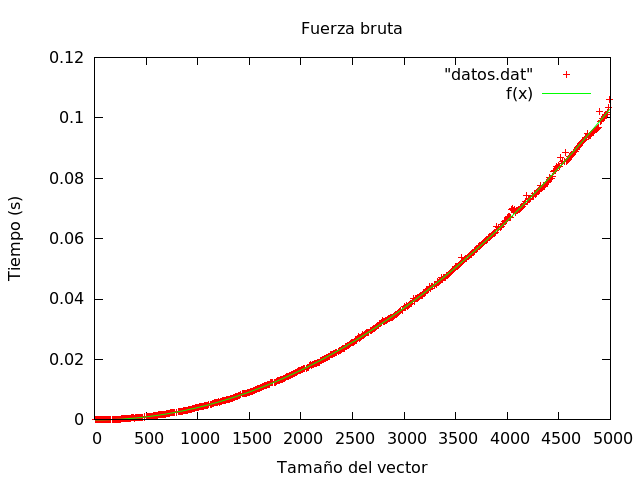
\includegraphics[width=1\textwidth]{../Opcional/Graficas/fuerza_bruta_bruno.png}
	\end{figure}
	\end{column}
\end{columns}
\end{frame}


\subsection{Divide y vencerás}
\begin{frame}{Divide y vencerás}
	\begin{columns}
		
		\begin{column}{4cm}
		\begin{block}{Algoritmo}
		Utilizamos el método de mezcla para contar el número de inversiones en cada sección.\\
		\end{block}	
		
		\begin{block}{Criterio}
		Dos elementos están invertidos si $i < j$ pero $v[i] > v[j]$\\
		\end{block}	
		\end{column}
			
		\begin{column}{6cm}
		\begin{exampleblock}{Ejemplo}
		\begin{figure}[h]
			\centering
			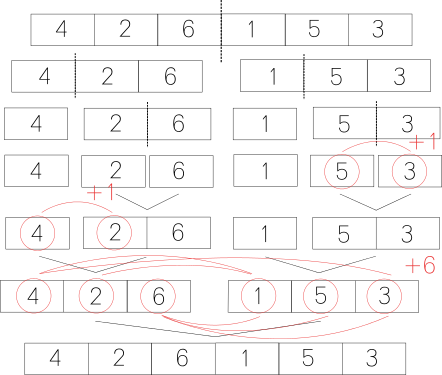
\includegraphics[width=1\textwidth]{Imagenes/esquema.png}
		\end{figure}
		\end{exampleblock}
		\end{column}
		
	\end{columns}
\end{frame}

\begin{frame}{Implementación}
\lstinputlisting[language=C++, firstline=112, lastline=128]{../Opcional/src/dyv.cpp}
\end{frame}

\begin{frame}{Eficiencia teórica}
\begin{block}{Recurrencia}
$$\left\lbrace
	\begin{array}{l}
	T(n) = \frac{n^2 - n}{2}\  si\ n \leq 2\\
	T(n) = 2T(\frac{n}{2}) + 2n\  si\ n > 2 \\
	\end{array}
	\right.$$\\
\end{block}

\begin{block}{Solución}
$$n=2^k \Rightarrow k = \log_2n$$
$$T(k) = 2^kT(1) + 2^kn$$
$$T(n) = n \cdot 0 + n^2$$
$$O(n^2)$$
\end{block}
\end{frame}

\begin{frame}{Eficiencia empírica}
\begin{figure}[h]
	\centering
		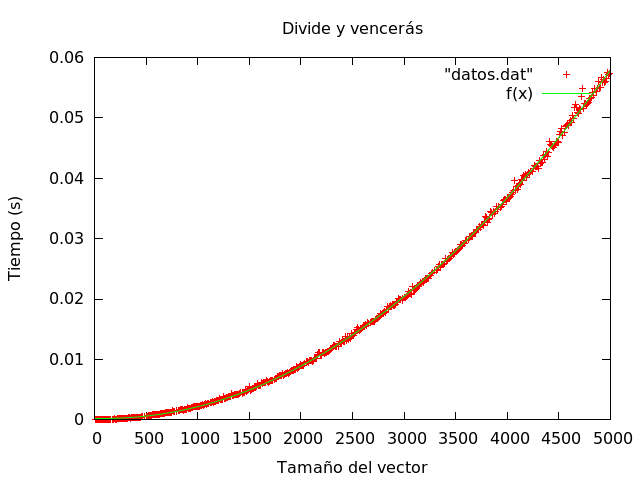
\includegraphics[width=0.6\textwidth]{../Opcional/Graficas/dyv_bruno.png}
\end{figure}

\begin{block}{Ajuste}
\begin{center}
$a = 2.6999 \cdot 10^{-9}$
$b = -8.47849 \cdot 10^{-7}$
$c = 0.000424603$
\end{center}
\end{block}
\end{frame}


\subsection{Divide y vencerás con mergesort}
\begin{frame}{Divide y vencerás con mergesort}
	\begin{columns}
		
		\begin{column}{4cm}
		\begin{block}{Algoritmo}
		Utilizamos el algoritmo de ordenación mergesort para contar el número de inversiones.\\
		\end{block}	
		
		\begin{block}{Criterio}
		Dos elementos están invertidos si $i < j$ pero $v[i] > v[j]$\\
		\end{block}	
		\end{column}
			
		\begin{column}{6cm}
		\begin{exampleblock}{Ejemplo}
		\begin{figure}[h]
			\centering
			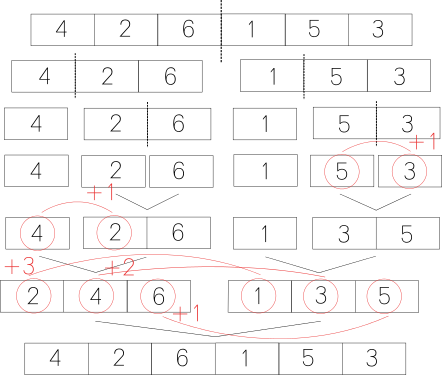
\includegraphics[width=1\textwidth]{Imagenes/esquema_merge.png}
		\end{figure}
		\end{exampleblock}
		\end{column}
		
	\end{columns}
\end{frame}

\begin{frame}{Implementación}
\lstinputlisting[language=C++, firstline=111, lastline=128]{../Opcional/src/dyv_mergesort.cpp}
\end{frame}

\begin{frame}{Eficiencia}
\begin{columns}
\begin{column}{5cm}
\begin{block}{Eficiencia teórica}
Tiene la misma eficiencia que mergesort, $O(n\log n)$
\end{block}

\begin{block}{Ajuste}
$a = 1.99872 \cdot 10^{-8}$
\end{block}
\end{column}

\begin{column}{6.5cm}
\begin{figure}[h]
	\centering
	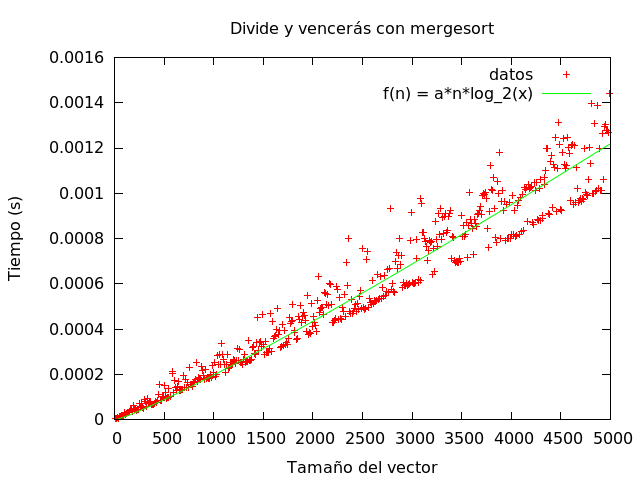
\includegraphics[width=1\textwidth]{../Opcional/Graficas/dyv_mergesort_bruno.png}
\end{figure}
\end{column}
\end{columns}
\end{frame}

\subsection{Comparación}
\begin{frame}{Comparación}
\begin{exampleblock}{Tabla comparativa}
\begin{table}
\begin{tabular}{|l|l|l|l|}
\multicolumn{1}{c}{\textbf{N}} & \multicolumn{1}{c}{\textbf{FUERZA BRUTA}} & \multicolumn{1}{c}{\textbf{DyV}} & \multicolumn{1}{c}{\textbf{MERGESORT}} \\
\hline
10                                                     & 5.372e-06                                                         & 5.01e-06                                                 & 4.475e-06                                                          \\
\hline
100                                                    & 4.3868e-05                                                        & 4.5584e-05                                               & 1.7295e-05                                                         \\
\hline
500                                                    & 0.00113                                                           & 0.000778726                                              & 8.8503e-05                                                         \\
\hline
1000                                                   & 0.0045925                                                         & 0.00247251                                               & 0.000218733                                                        \\
\hline
1500                                                   & 0.0106898                                                         & 0.00567031                                               & 0.000289624                                                        \\
\hline
2000                                                   & 0.0171023                                                         & 0.0094678                                                & 0.000382864                                                        \\
\hline
\end{tabular}
\end{table}
\end{exampleblock}
\end{frame}

\begin{frame}
\begin{figure}[h]
	\centering
	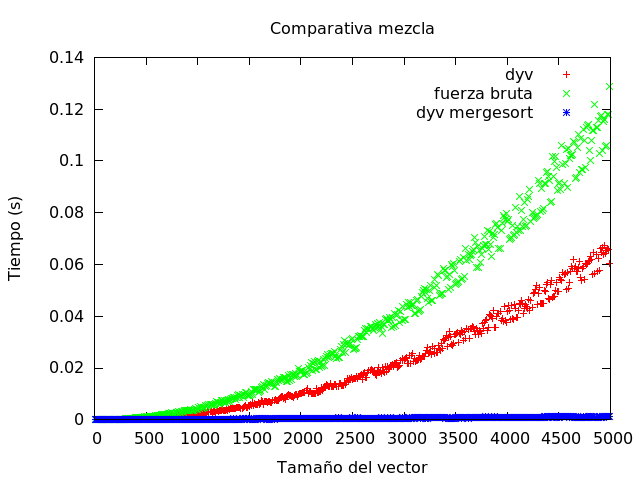
\includegraphics[width=1\textwidth]{../Opcional/Graficas/comparativa.png}
\end{figure}
\end{frame}
\end{document}
